\section{Построение МТЧ СНС и результаты ее исследования}

\begin{enumerate}
	\item Синтезировать закон управления (ЗУ) вида $u(t) = K_g g(t) + K x(t)$, который должен обеспечивать системе:
	\begin{equation}\label{eq_mod_control}
		\begin{cases}
			\dot x(t, q) = F(q) x(t,q) + G(q) g(t);\\
			y(t, q) = C(q) x(t,q)
		\end{cases},
	\end{equation} 
	где $F(q) = A(q) - B(q) K, G(q) = B(q) K_g$,
	образованной объединением НОУ и ЗУ равенство входа $g(t)$ и выхода $y(t)$ в неподвижном состоянии при номинальных значениях параметров с помощью:
	\begin{enumerate}
		\item матрицы $K_g$ прямой связи по входу $g(t)$;
		\item матрыцы $K$ обратной связи по состоянию $x(t)$
	\end{enumerate}
	распределение мод Баттерворта с характеристической частотой $\omega_0 = 3 c^{-1}$;
	\item Построить МТЧ спроектированной системы по каждому из параметров и для значения $|\Delta q_j| = 0.2$;
	\item Выделить доминирующие параметры по степени их влияния на величину $\sigma$ перерегулирования и длительнсоти $t_\text{п}$ переходного процесса.
\end{enumerate}

\subsection{Синтез закона модального управления}


Замкнутая система~\ref{eq_mod_control} образована агрегированием ОУ~\ref{eq_iso_coc} и регулятора, реализующего закон управления:
\begin{equation}\label{reg}
	u(t) = K_g g(t) + K x(t)
\end{equation}
в виде прямой связи (ПС) по внешнему воздействию и отрицательной обратной связи (ОС) по вектору состояния ОУ, матрицы которого $K_g$ и $K$ просинтезированы для случая номинальной версии ОУ.

Перед началом расчета матриц коэффициентов регулятора~\ref{reg} убедимся, что система~\ref{eq_iso_coc} обладает свойством управляемости. Для этого найдем матрицу управляемости и ее определитель

\begin{equation}
	U = 
	\begin{bmatrix}
	B & A B
	\end{bmatrix}
	=
	\begin{bmatrix}
	0  &  1\\         
	1 & - 1.9666667
	\end{bmatrix}
\end{equation}
\begin{equation}
	det(U) = -1
\end{equation}
Номинальна система ОУ~\ref{eq_iso_coc} полностью управляема, так как матрица управляемости $U$ не вырождена. $rang(U) = 2$ и равен порядку систему.

Для придания матрице $F = A - BK$ распределения мод Баттерворта с характеристической частотой $\omega_0 = 3 c^{-1}$ составим эталонную модель ОУ
\begin{equation}
	\begin{cases}
		\dot \xi (t) = \Gamma \xi(t)\\
		v (t) = H \xi(t)
	\end{cases}
\end{equation}
где $\Gamma$ и $H$~--- матрицы состояния и выхода эталонной системы.

Решим стандартный полином Баттерворта второго порядка
\begin{equation}
\lambda^2 + 1.414 \omega_0 \lambda + \omega_0^2 = 0
\end{equation}
\begin{equation}
\lambda^2 + 4.242 \lambda + 9 = 0,
\end{equation}
корни которого $\lambda_{1,2} = - 2.121 \pm j 2.1216406 $


Определим матрицы состояния и выхода эталонной модели. Так как корни желаемого полинома получились комплексные, то матрица $\Gamma$ примет вид
\begin{equation}
	\Gamma = 
	\begin{bmatrix}
	-\alpha & \beta\\
	-\beta & -\alpha
	\end{bmatrix}
	=
	\begin{bmatrix}
	 - 2.121    &    2.1216406  \\
	- 2.1216406  &- 2.121 	
	\end{bmatrix}
\end{equation}

Матрица $H$ выбирается из условия полной наблюдаемости матриц $\Gamma$ и~$H$
\begin{equation}
	H = 
	\begin{bmatrix}
	1 & 0
	\end{bmatrix}
\end{equation}

Матрицу коэффициентов ОС $K$ найдем из решения системы уравнений
\begin{equation}
	\begin{cases}
	 B H = M \Gamma - A M\\
	 K = - H M^{-1}
	\end{cases}
\end{equation}

Вычислим матрицу преобразования $M$
\begin{equation}
	M = 
	\begin{bmatrix}
	  - 0.0998304 &   0.1311712\\
	  - 0.0665578 & - 0.4900185  	
	\end{bmatrix}
\end{equation}

Найдем матрицу коэффициентов $K$

\begin{equation}\label{Kq}
	K = 
	\begin{bmatrix}
	 8.5  &  2.2753333
	\end{bmatrix}
\end{equation}

Запишем матрицу замкнутой системы $F$ при номинальных значениях параметров $q_j$
\begin{equation}
	F = 
	\begin{bmatrix}
	   0 &    1\\     
	- 9&  - 4.242
	\end{bmatrix}
\end{equation}

Найдем матрицу коэффициентов ПС $K_g$ из следующего выражения

\begin{equation}
	K_g = - (C F^{-1} B)^{-1}
\end{equation}
\begin{equation}
	K_g = 270
\end{equation}

Тогда матрица $G$ принимает вид
\begin{equation}
	G = B K_g = 
	\begin{bmatrix}
	0\\ 
	270
	\end{bmatrix}
\end{equation}

Смоделируем полученную систему в пакете прикладных математических программ Scilab, подав в качестве входного сигнала единичное ступенчатое воздействие
\begin{figure}[h!]
	\centering
	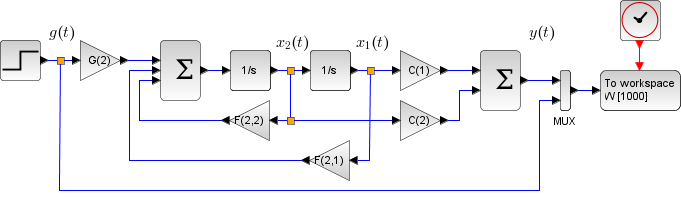
\includegraphics[width=1\textwidth]{mod_control.png}
	\caption{Схема моделирования замкнутой системы~\ref{eq_mod_control}}
	\label{fig:mod_control}
\end{figure}
\newpage


\begin{figure}[h]
	\centering
	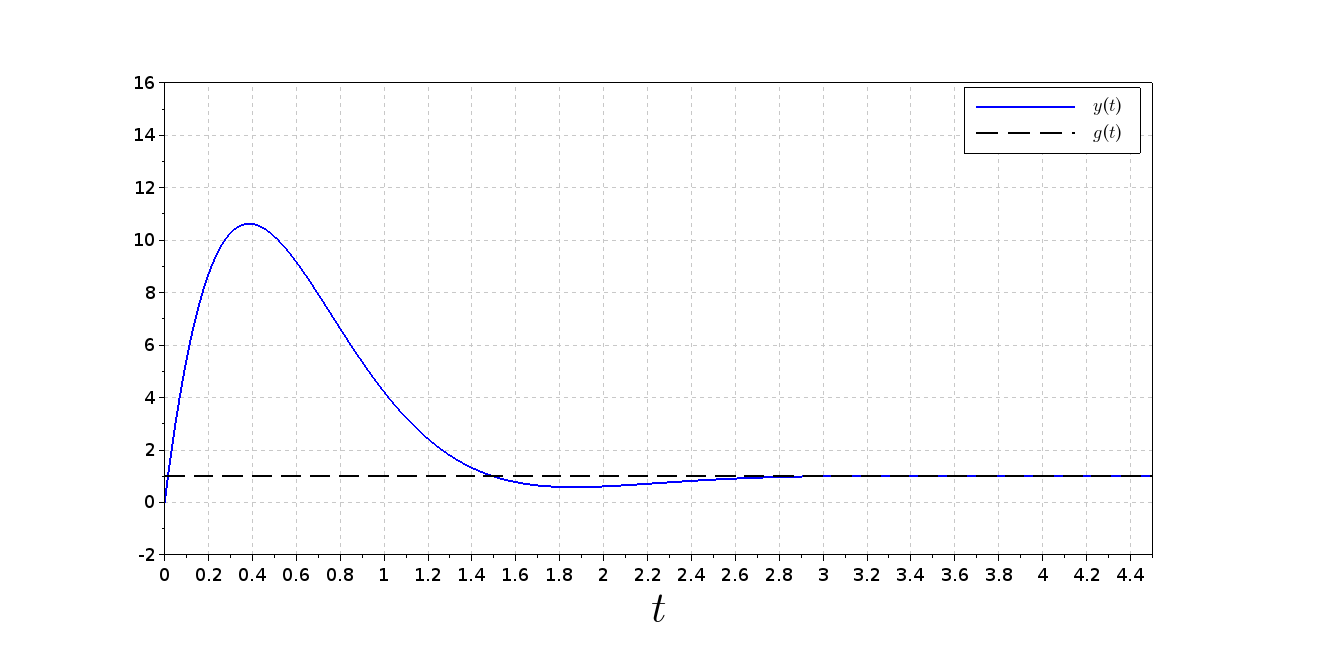
\includegraphics[width=1\textwidth]{res_mod_control.png}
	\caption{Переходная характеристика замкнутой системы~\ref{eq_mod_control}}
	\label{fig:mod_control}
\end{figure}

Таким образом, система обеспечивает равенство входа $g(t)$ и выхода $y(t)$ в неподвижном состоянии при номинальных значениях параметров $q_j$.

\subsection{Построение МТЧ спроектированной системы для каждого из параметров $q_j$}

Введем обозначения
\begin{align*}
&F_{q_j} = \cfrac{\partial{F(q)}}{\partial{q_j}} \bigg|_{q=q_0};
G_{q_j} = \cfrac{\partial{G(q)}}{\partial{q_j}} \bigg|_{q=q_0};
&F(q)|_{q=q_0} = F;
G(q)|_{q=q_0} = G;
\end{align*}

Подобно тому, как МТЧ строилась ранее, МТЧ замкнутой системы (ЗС)
\begin{equation}\label{eq_mts_ls_3}
	\begin{cases}
		\dot \sigma_j(t) &= F \sigma_j(t) + F_{q_j} x(t) + G_{q_j} g(t); 
		\sigma_j (0) = 0\\
		\eta_j (t) &= C \sigma_j (t) + C_{q_j} x(t)
	\end{cases}
\end{equation}

Пользуясь матрицами НОУ~\ref{Aq}~и~\ref{Bq}, рассчитаем матрицу $F(q) = A(q) - B(q) K$, где $K$~--- рассчитанная матрица коэффициентов ОС~\ref{Kq} (матрица $F(q)$ изображена транспонированной из соображений компактности записи)
\begin{equation}
	F(q) =
	\begin{bmatrix}
		0 & - \cfrac{(1+q_4)(1+q_7)}{2(1+q_3)(1+q_6)} - 8.5 \\
		1 & - \cfrac{20(1+q_3)(1+q_7)+3.6(1+q_4)(1+q_6)}{12(1+q_3)(1+q_6)} - 2.2753333
	\end{bmatrix}^T
\end{equation}

Рассчитаем матрицы для системы~\ref{eq_mts_ls_3} (матрицы $F_{q_j}$ приведены без операции транспонирования)

\begin{align}\label{mxs_sense}
&F_{q_{1,2}} = 
\begin{bmatrix}
0 & 0\\
0 & 0
\end{bmatrix};
F_{q_3} = 
\begin{bmatrix}
0 & 0\\
\cfrac{1}{2} & \cfrac{36}{120}
\end{bmatrix};
F_{q_4} = 
\begin{bmatrix}
0 & 0\\
- \cfrac{1}{2} & - 3.6
\end{bmatrix};
F_{q_6} = 
\begin{bmatrix}
0 & 0\\
\cfrac{1}{2} & \cfrac{20}{12}
\end{bmatrix};\\
&F_{q_7} = 
\begin{bmatrix}
0 & 0\\
- \cfrac{1}{2} & - \cfrac{20}{12}
\end{bmatrix};
G_{q_{1,2,3,4,6,7}} = 
\begin{bmatrix}
0\\
0
\end{bmatrix};
C_{q_1} = 
\begin{bmatrix}
0 & \cfrac{1}{4}
\end{bmatrix};
C_{q_2} = 
\begin{bmatrix}
\cfrac{1}{30} & 0
\end{bmatrix};\\
&C_{q_3} = 
\begin{bmatrix}
- \cfrac{1}{30} & - \cfrac{1}{4}
\end{bmatrix};
C_{q_4} = 
\begin{bmatrix}
0 & 0
\end{bmatrix};
C_{q_6} = 
\begin{bmatrix}
- \cfrac{1}{30} & - \cfrac{1}{4}
\end{bmatrix};
C_{q_7} = 
\begin{bmatrix}
0 & 0
\end{bmatrix};
\end{align}

Матрицы эквивалентны матрицам ОУ, так как матрица управления $B$ не зависит от параметров $q_j$.

Сконструируем агрегированную систему с составным вектором \newline $\tilde{x}_j=col\{x_j,\sigma_j\}$ размерности $ \dim \tilde{x} = 2n$, которая объединением \ref{eq_mod_control} и \ref{eq_mts_ls_3}, получает представление
\begin{align}\label{rang_system_3}
	\dot{\tilde{x}}_j (t) &= \tilde{F}_j \tilde{x}_j (t) + \tilde{G}_j g(t); 
	\tilde{x}_j (0) = col \{x(0), 0\}\\
	x(t) &= \tilde{C}_{x_j} \tilde{x}_j;\\
	y(t) &= \tilde{C}_j \tilde{x}_j (t);\\
	\sigma_j (t) &= \tilde{C}_{\sigma_j} \tilde{x}_j (t);\\
	\eta_j (t) &= \tilde{C}_{\eta_j} \tilde{x}_j (t)
\end{align}
где 
\begin{align*}
	&\tilde{{F}} =
	\begin{bmatrix}
	{F} & 0\\
	{F}_{q} & {F}
	\end{bmatrix},
	\tilde{{G}} = 
	\begin{bmatrix}
	{G}\\
	{G}_{q}
	\end{bmatrix},
\end{align*}

Структура матриц выхода $C$ совпадают с матрицами системы~\ref{rang_system}.
Составим матрицы агрегированной системы~\ref{rang_system_3}

\begin{align*}
	&\tilde{{F_{1,2}}} =
	\begin{bmatrix}
		  0   & 1     &  0  &  0\\     
		- 9 & - 4.242 &   0 &   0 \\    
		0   & 0  &     0  &  1     \\
		0   & 0 &    - 9 & - 4.242  	
	\end{bmatrix};
	\tilde{{F_3}} =
	\begin{bmatrix}
    0&     1&       0&    0.     \\
	- 9&   - 4.242 &  0&    0.    \\ 
	0&     0&       0&    1.    \\ 
	0.5 &  0.3 &  - 9&  - 4.242  
	\end{bmatrix};\\
	&\tilde{{F_4}} =
	\begin{bmatrix}
	    0&     1&       0&    0.     \\
		- 9&   - 4.242 &  0&    0.    \\ 
		0&     0&       0&    1.    \\ 
		-0.5 &  -0.3 &  - 9&  - 4.242  
	\end{bmatrix};
	\tilde{{F_6}} =
	\begin{bmatrix}
		0&     1&       0&    0.     \\
		- 9&   - 4.242 &  0&    0.    \\ 
		0&     0&       0&    1.    \\ 
		0.5  &  1.6666667 &  - 9&  - 4.242  
	\end{bmatrix};\\
	&\tilde{{F_7}} =
	\begin{bmatrix}
		0&     1&       0&    0.     \\
		- 9&   - 4.242 &  0&    0.    \\ 
		0&     0&       0&    1.    \\ 
		-0.5  &  -1.6666667 &  - 9&  - 4.242  
	\end{bmatrix};
	\tilde{{G}} =
	\begin{bmatrix}
		0\\1\\0\\0
	\end{bmatrix};\\
	&\tilde{{C}}_{\eta_1} =
	\begin{bmatrix}
		0&0.25&0.0333333 &   0.25\\
	\end{bmatrix}
	\tilde{{C}}_{\eta_2} =
	\begin{bmatrix}
		0.0333333&0&0.0333333 &   0.25\\
	\end{bmatrix}\\
	&\tilde{{C}}_{\eta_{3,7}} =
	\begin{bmatrix}
		-0.0333333&-0.25&0.0333333 &   0.25\\
	\end{bmatrix}
	\tilde{{C}}_{\eta_{4,7}} =
	\begin{bmatrix}
	0&0&0.0333333 &   0.25\\
	\end{bmatrix}
\end{align*}


Смоделируем полученную систему в пакете прикладных математических программ Scilab, подав в качестве входного сигнала единичное ступенчатое воздействие
\begin{figure}
	\centering
	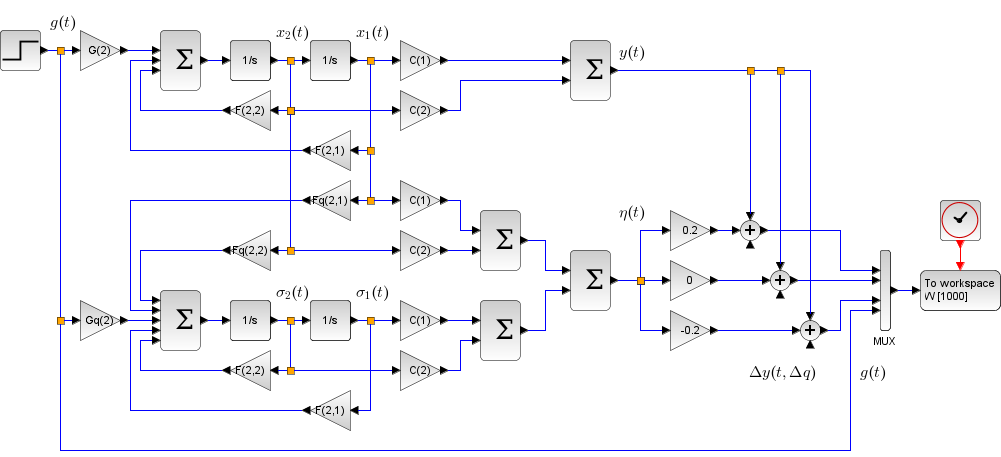
\includegraphics[width=1\textwidth]{mod_control_mts.png}
	\caption{Схема моделирования МТЧ дополненной НОУ~\ref{eq_mod_control}}
	\label{fig:mod_control_mts}
\end{figure}

\begin{figure}
	\centering
	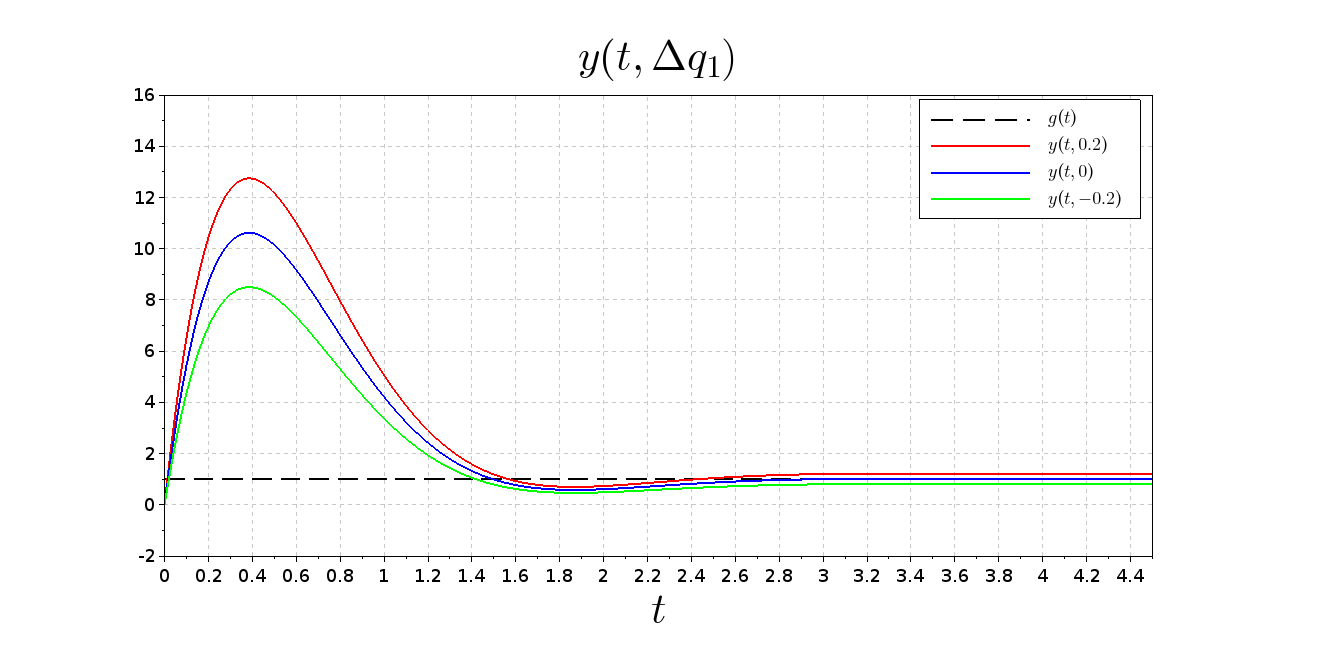
\includegraphics[width=1\textwidth]{res_3_q1.png}
	\caption{Переходные процессы при вариации параметра $q_1$}
	\label{fig:res_3_q1}
\end{figure}

\begin{figure}
	\centering
	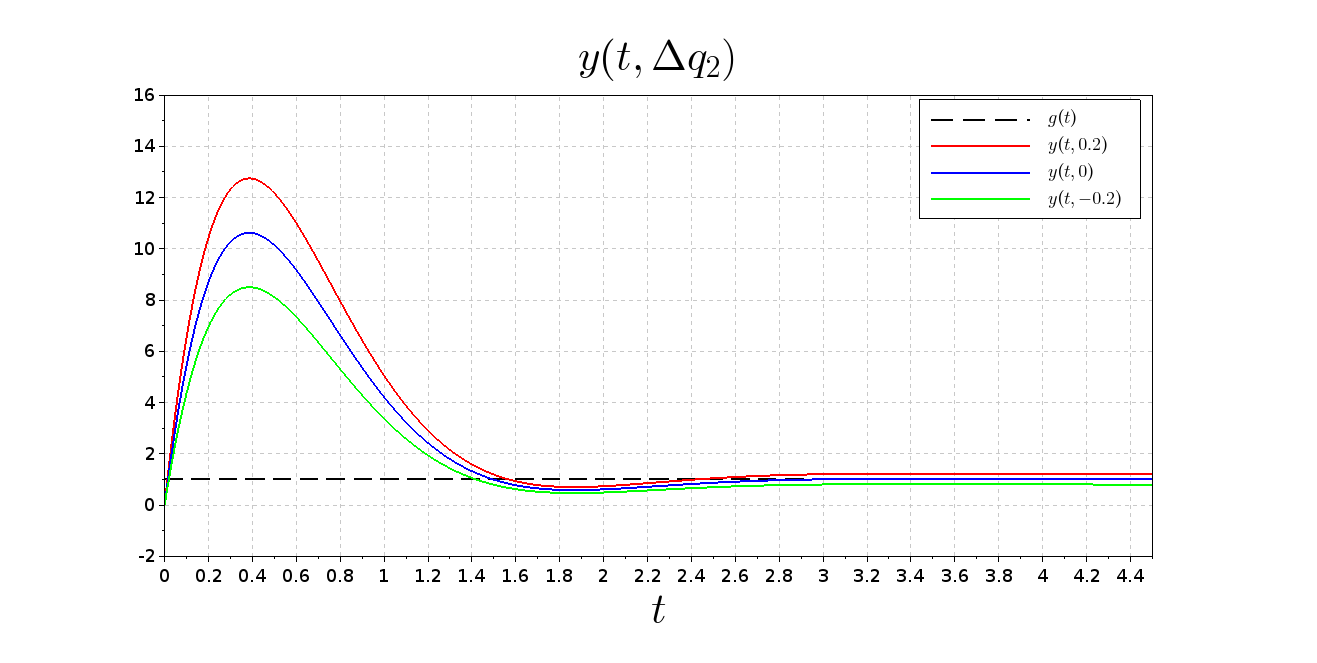
\includegraphics[width=1\textwidth]{res_3_q2.png}
	\caption{Переходные процессы при вариации параметра $q_2$}
	\label{fig:res_3_q2}
\end{figure}
\begin{figure}
	\centering
	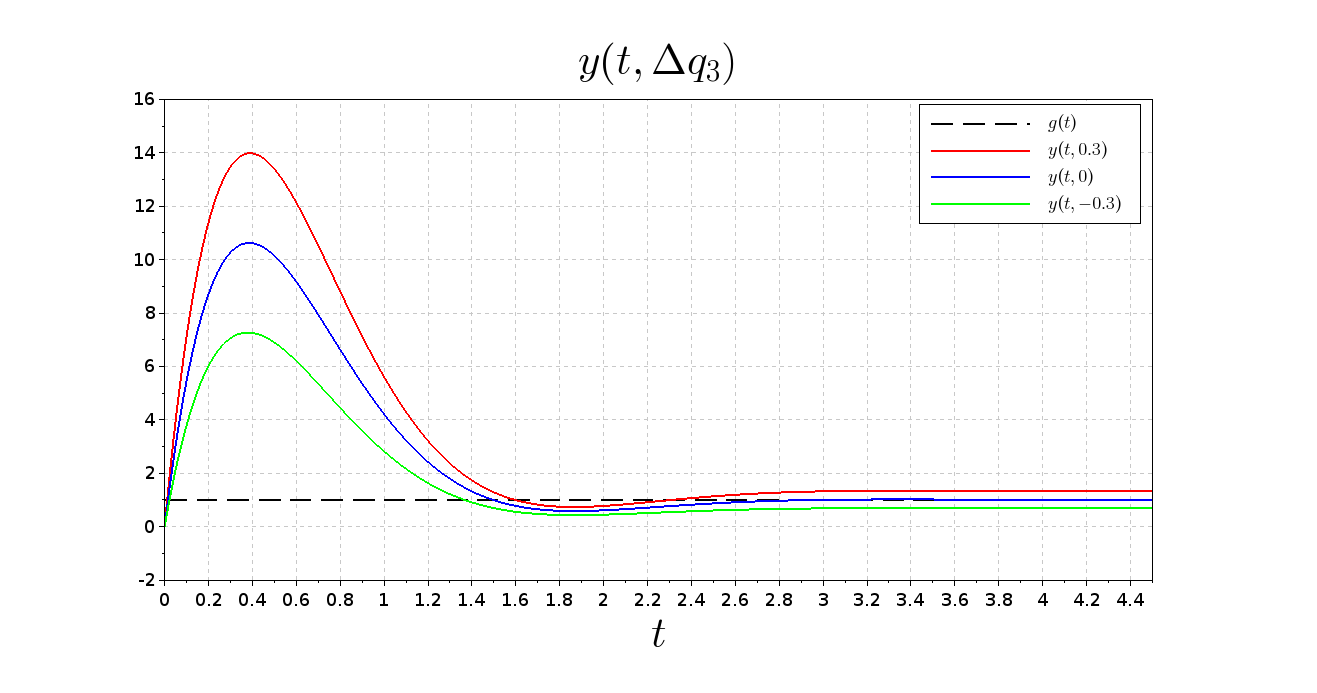
\includegraphics[width=1\textwidth]{res_3_q3.png}
	\caption{Переходные процессы при вариации параметра $q_3$}
	\label{fig:res_3_q3}
\end{figure}
\begin{figure}
	\centering
	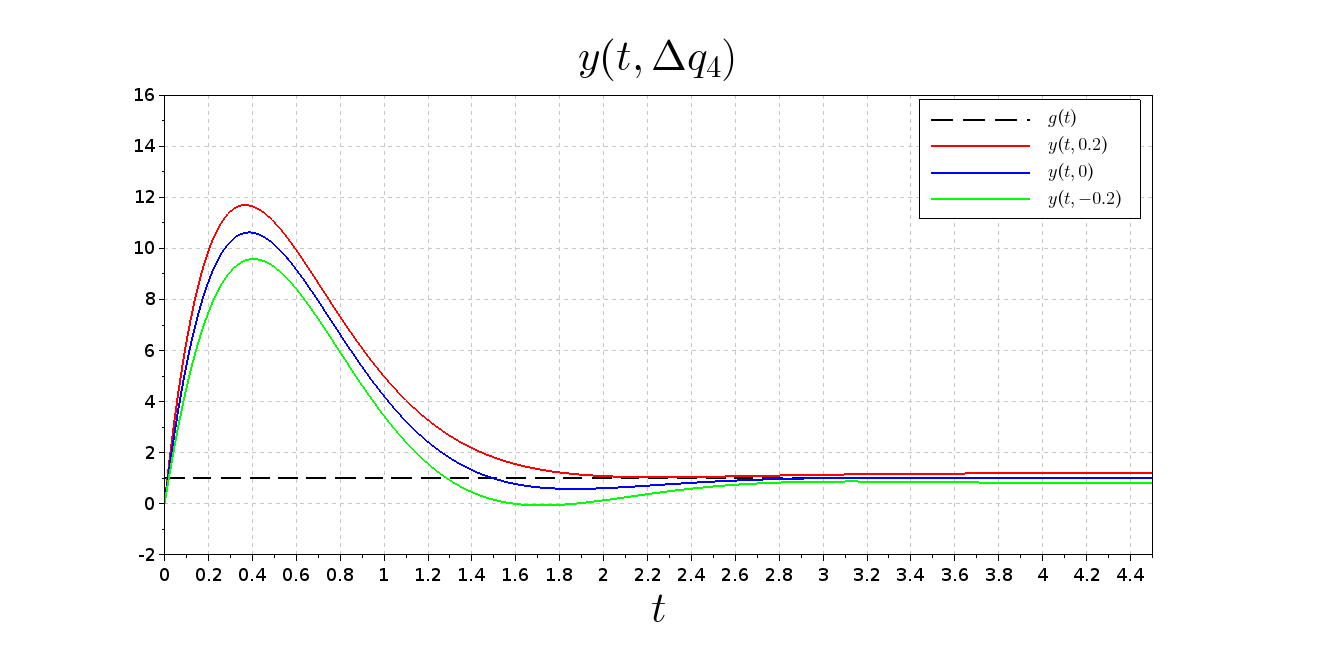
\includegraphics[width=1\textwidth]{res_3_q4.png}
	\caption{Переходные процессы при вариации параметра $q_4$}
	\label{fig:res_3_q4}
\end{figure}
\begin{figure}
	\centering
	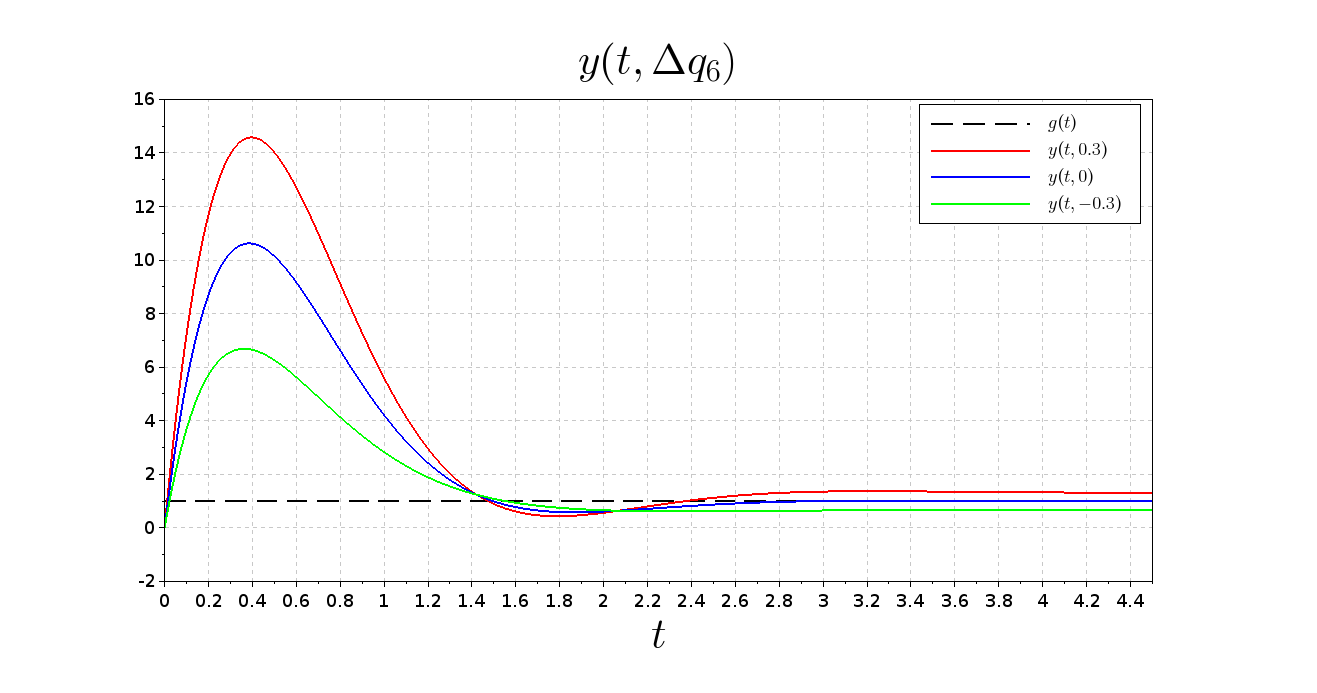
\includegraphics[width=1\textwidth]{res_3_q6.png}
	\caption{Переходные процессы при вариации параметра $q_6$}
	\label{fig:res_3_q6}
\end{figure}
\begin{figure}
	\centering
	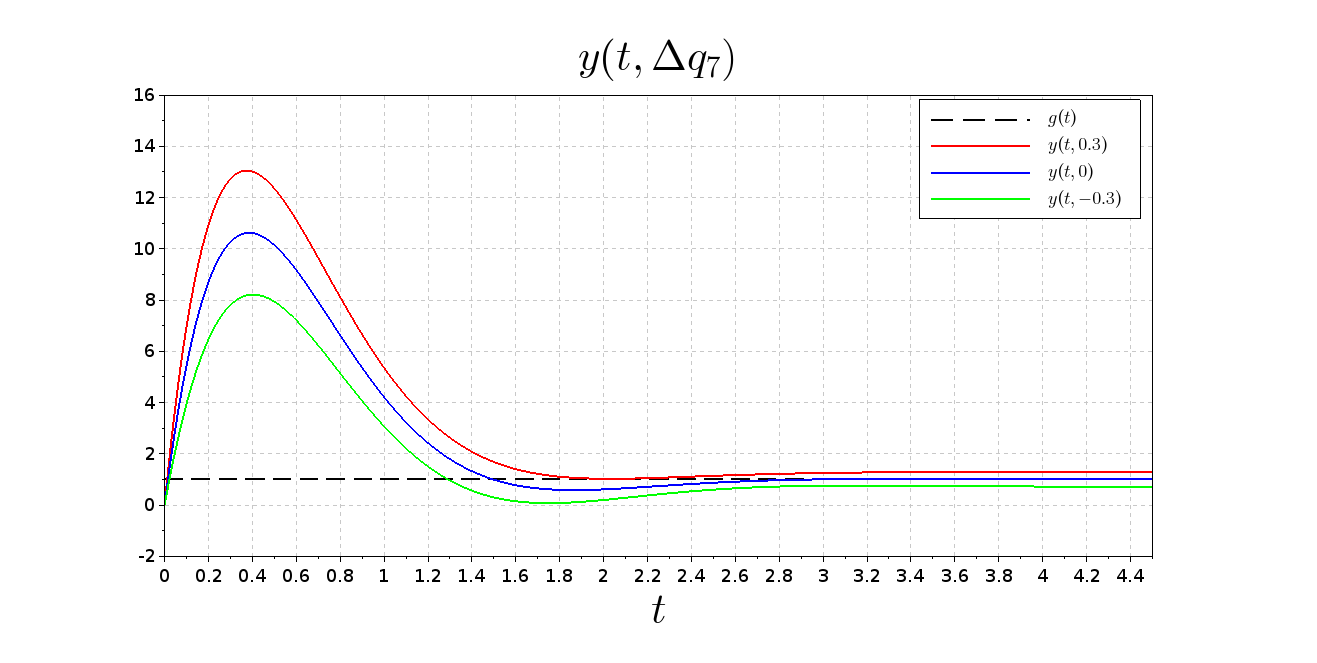
\includegraphics[width=1\textwidth]{res_3_q7.png}
	\caption{Переходные процессы при вариации параметра $q_7$}
	\label{fig:res_3_q7}
\end{figure}

\newpage
\subsection{Определение доминирующих параметров}

Занесем полученные из построенных графиков значения перерегулирования $\sigma$ и времени переходного процесса  $t_{\text{п}}$ в таблицу~\ref{t:dom}.

\begin{table}[h!]
	\centering
	\caption{Значения переререгулирования и времени преходного процесса для варьируемых парметров $q_j$}
	\label{t:dom}
	\begin{tabular}{|c|c|c|c|c|c|c|}
		\hline
		\multirow{2}{*}{Параметр} & \multicolumn{3}{c|}{\begin{tabular}[c]{@{}c@{}}Перерегулирование\\ $\sigma$, \%\\ при $\Delta q =$\end{tabular}} & \multicolumn{3}{c|}{\begin{tabular}[c]{@{}c@{}}Вр.перех.процесса\\ $t_\text{п}$, сек.\\ при $\Delta q =$\end{tabular}} \\ \cline{2-7} 
		& 0.2 & 0 & -0.2 & 0.2 & 0 & -0.2 \\ \hline
		$q_1$ & 1275 & \multirow{6}{*}{1062} & 850 & 2.78 & \multirow{6}{*}{2.72} & 2.72 \\ \cline{1-2} \cline{4-5} \cline{7-7} 
		$q_2$ & 1275 &  & 549 & 2.72 &  & 2.72 \\ \cline{1-2} \cline{4-5} \cline{7-7} 
		$q_3$ & 1286 &  & 839 & 2.69 &  & 2.76 \\ \cline{1-2} \cline{4-5} \cline{7-7} 
		$q_4$ & 1169 &  & 958 & 3.03 &  & 3.64 \\ \cline{1-2} \cline{4-5} \cline{7-7} 
		$q_6$ & 1326 &  & 799 & 2.67 &  & 2.92 \\ \cline{1-2} \cline{4-5} \cline{7-7} 
		$q_7$ & 1224 &  & 901 & 2.82 &  & 2.65 \\ \hline
	\end{tabular}
\end{table}

Рассчитаем отклонения значений перерегулирования $\Delta \sigma$ и времени переходного процесса $t_{\text{п}}$ характеристик системы при вариациях параметров $q_j$ от номинальной характеристики и занесем их в таблицу~\ref{t:res}.

\begin{table}[h!]
	\centering
	\caption{Отклонения характеристик системы с варьируемыми параметрами от номинальной системы}
	\label{t:res}
	\begin{tabular}{|c|c|c|c|c|}
		\hline
		\multirow{2}{*}{Параметр} & \multicolumn{2}{c|}{\begin{tabular}[c]{@{}c@{}}$\Delta \sigma$, \%\\ при $\Delta q = $\end{tabular}} & \multicolumn{2}{c|}{\begin{tabular}[c]{@{}c@{}}$\Delta t_\text{п}$, сек.\\ при $\Delta q = $\end{tabular}} \\ \cline{2-5} 
		& 0.2 & -0.2 & 0.2 & -0.2 \\ \hline
		$q_1$ & 213 & 212 & 0.06 & 0 \\ \hline
		$q_2$ & 221 & 514 & 1 & 1 \\ \hline
		$q_3$ & 222 & 225 & 2.03 & 1.96 \\ \hline
		$q_4$ & 104 & 107 & 2.69 & 2.08 \\ \hline
		$q_6$ & 260 & 267 & 4.05 & 3.8 \\ \hline
		$q_7$ & 157 & 166 & 4.9 & 5.07 \\ \hline
	\end{tabular}
\end{table}
где
\begin{equation}
	\Delta \sigma_{\Delta q = \pm 0.2} = |\sigma_{\Delta q = \pm 0.2} - \sigma_{\Delta q = 0}|
\end{equation}

\begin{equation}
	\Delta t_{\text{п}, \Delta q = \pm 0.2} = |t_{\text{п}, \Delta q = \pm 0.2} - t_{\text{п}, \Delta q = 0}|
\end{equation}

Выделим доминирующие параметры по степени их влияния на величину $\sigma$ перерегулирования и длительнсоти $t_\text{п}$ переходного процесса

	
\begin{enumerate}
	\item Влияние на величину перерегулирования (в порядке уменьшения)
		\begin{enumerate}
			\item при $\Delta q = 0.2$: 
				$q_6$,
				$q_3$,
				$q_2$,
				$q_1$,
				$q_7$,
				$q_4$;					
			\item при $\Delta q = -0.2$
				$q_2$,
				$q_6$,
				$q_3$,
				$q_1$,
				$q_7$,
				$q_4$;					
		\end{enumerate}	
	\item Влияние на время переходного процесса(в порядке уменьшения)
		\begin{enumerate}
			\item при $\Delta q = \pm 0.2$: 
			$q_7$,
			$q_6$,
			$q_4$,
			$q_3$,
			$q_2$,
			$q_1$;					
		\end{enumerate}	
\end{enumerate}

\newpage